% carried verbatim from the v2 tree (results.tex); NOT part of this session's deliverable.
\begin{figure*}[tp]\centering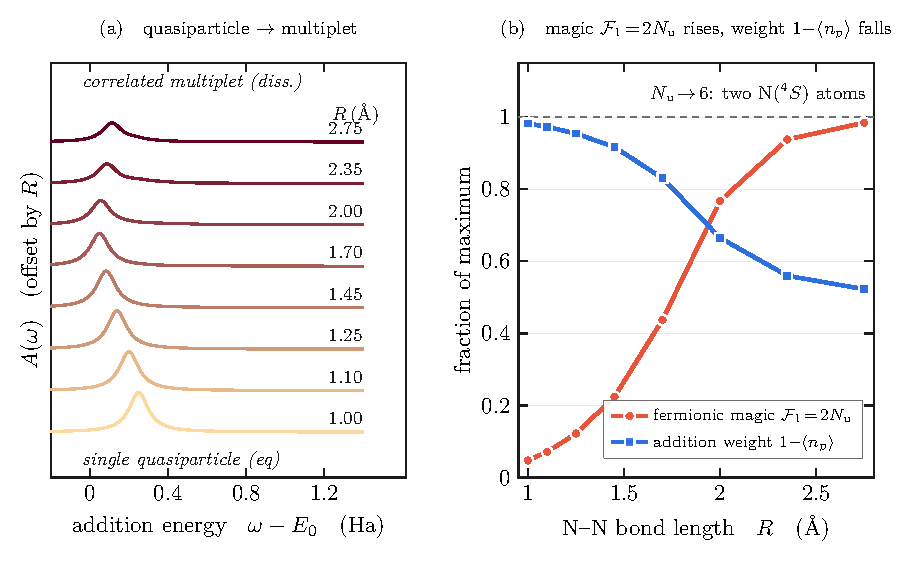
\includegraphics[width=\linewidth]{figs/fig_hero.pdf}
\caption{\textbf{Magic and multireference character in $\mathrm{N_2}$ dissociation.} (a)~The exact
addition spectral function $A(\omega)$ (orbital-projected, CAS(6,6), cc-pVDZ) along the triple-bond
stretch, offset by $R$: the sharp coherent quasiparticle peak at equilibrium ($R=1.0$~\AA) broadens
into a correlated multiplet on dissociation as its spectral weight collapses. (b)~Two physically
independent quantities along the same coordinate. The fermionic magic obeys the \emph{exact} identity
$\mathcal F_1=2N_{\mathrm u}$ [Eq.~\eqref{eq:collapse}, verified to $<10^{-13}$], so a single curve carries both: it rises
with the orbital-rotation-invariant multireference count---the effective number of unpaired electrons
$N_{\mathrm u}=\sum_i n_i(2-n_i)$ from the natural-orbital occupations $n_i$, approaching its atomic limit of $6$
(the two triplet $\mathrm{N}(^4S)$ atoms) as the bond fully breaks. The integrated addition weight $\int A^{+}d\omega=1-\langle\hat n_p\rangle$
(from panel a) falls from $0.98$ to $0.52$ over the same stretch; the two cross as the bond
breaks. The active-space CASCI energies are converged to $1.1\times10^{-13}$~Ha, which is a
convergence check and not a validation against an independent method
(Sec.~\ref{sec:scope:mol}).}\label{fig:hero}\end{figure*}
